
\subsection{Grid Computing}

Din punct de vedere arhitectural, protocolul din cadrul unei retele grid este format din 5
layer-ere. Acestea sunt detaliate si in Figura 3.1 \cite{foster2008cloud}.

\begin{figure*}[ht] \centering
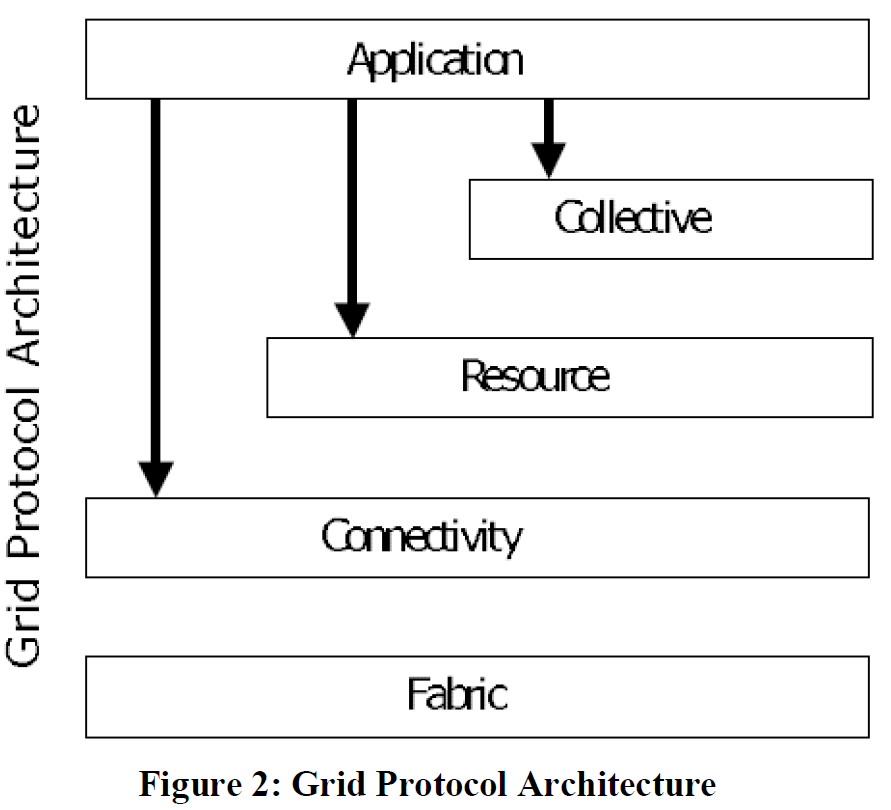
\includegraphics[width=0.6\textwidth]{img/grid.png}
\caption{Arhitectura protocolului grid} \end{figure*}


\begin{itemize}

    \item Connectivity Layer. Este nivelul in care protocolul GSI( Grid Security Infrastructure)
        guverneaza fiecare tranzactie de date din reteaua grid. 
\item Resource Layer. In cadrul acestui nivel este definit protocolul pentru descoperirea,
    publicarea si monitorizarea resurselor individuale. Protocolul folosit este GRAM (Grid Resource
    Acces and Management), acesta poate aloca, controla si monitoriza folosirea resurselor. 
\item Collective Layer. Acest nivel se ocupa cu planificarea si monitorizarea resurselor pentru
    servicii. Serviciile nu sunt asociate cu unei resurse specifice, astfel ca acest nivel se
    concentreaza pe interactiunea dintre resurse.
\item Application Layer. Acest nivel este reprezentat de aplicatiile pe care userul decide sa le
    execute.
\item Fabric Layer. Acest nivel este nivelul hardware, mai exact resursele hardware ale
    sistemelor, procesor, memorie, etc.
\end{itemize}

Grid computing execute in taskuri care sunt introduse intr-o coada de executie. Aceste taskuri cand
sunt rulate acapareaza complet resursele sitemului. Din aceasta cauza latenta retelor grid este
destul de mare, deoarece pana un task nu este executat, celelate ramana intr-o stare de asteptare.

\subsection{Cloud Computing}

Din punt de vedere arhitectural, protocolul din cadrul unei retele clod este mai simplu decat cel
din reteau de tip grid, fiind format din 5 layer-ere. Acestea sunt detaliate si in Figura 3.2.


\begin{itemize}
 
\item Fabric Layer. Acest nivel este identic ca cel de la grid, astfel este compus din resursele hardware ale
    sistemelor, procesor, memorie, etc.
\item Unified Resource Layer. Aest nivel contine resursele care au fost abstractizate (deobicei
    prin virtualizare) pentru a putea fi expuse unor nivele superioare. 
\item Platform Layer. Acest nivel adauga un set de API-uri si servicii peste nivelul de resurse
    unificate pentru a crea un mediu de dezvoltare necesar aplicatiilor de tip user level.
\item Application Layer. Acest nivel este la fel ca si in cazul retelor de tip grid, fiind
    constituit din aplicatiile utilizatorilor.

\end{itemize}


\begin{figure*}[ht] \centering
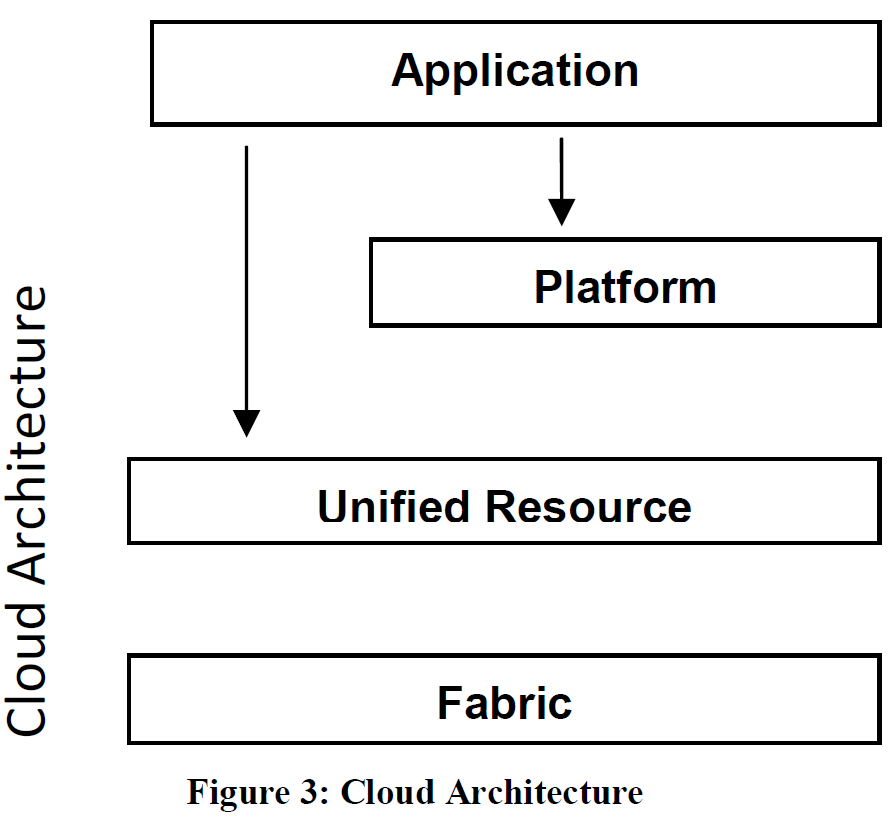
\includegraphics[width=0.6\textwidth]{img/cloud.png}
\caption{Arhitectura protocolului cloud } \end{figure*}


Cloud computing are resursele comune intre utilizatori. Din aceasta cauza, latenta aplicatiilor
este mult imbunatatita deoarece mai multe taskuri pot rula in acelasi timp. 


Desi cloud computing poate pune la dispozitie resurse masive intr-un timp foarte mic, cea mai mare
problema o reprezinta securitate. Prima problema a securitatii o constituie locatia fizica a
masinilor care fac parte din cloud, deoarece datele sensibile pot fi accesate de terti. 

Din acest motiv, organizatiile mari care au nevoie de executia programelor pe date sensibile au
construit propriile sisteme de tip grid. Un alt avantaj il consituie faptul ca nu necesita
conexiune la internet precum cloud pentru a putea rula taskuri in retea \cite{rings2009grid}.


